\chapter{Introduction}
\section{Background: Energy storage}
The demand for ever improving energy storage solutions is driven by both commercial interests and urgent societal need.
In order to curtail \ce{CO2} emissions and limit the impact of global warming, a shift from fossil-fuel based energy generation towards renewable energy is vital.\cite{Goodenough2013}
Unfortunately, a characteristic of many renewable energy sources, such as wind and solar energy, is the intermittent nature of its generation.\cite{Goodenough2010a}
As such, it is necessary to decouple the generation and consumption of the energy produced by these means via intermediate storage.

Vehicle electrification may displace conventional combustion engine driven transport, another major source of greenhouse gases and pollution.
While some commercial success has being enjoyed for electric vehicles in recent years, safety concerns and insufficient energy density to overcome the ``range anxiety'' of most consumers demands further development of battery technologies for widespread adoption of electric vehicles to occur.

Finally, consumer demand for increasingly powerful, thin, and light portable electronics with larger times between charges has pushed current battery chemistries to their limits.
With the majority of developments in batteries for portable electronics in recent years arising not from improvements in their chemistries, but by improved manufacturing processes with diminishing returns, the need for a fundamentally different battery chemistry may arise in the near future.
Indeed, in recent years a number of manufacturers have, in a drive to yield more performance from the same fundamental chemistries, produced cells which ultimately proved to be unsafe.\cite{Loveridge2018}

Each of the above use cases will prioritise different properties in their energy storage solutions. 
While safety and energy density are paramount in portable electronics and electric vehicles, low cost is the primary driver in load-levelling applications.


\newpage
\section{Li-ion Batteries}
\renewcommand{\thefootnote}{\fnsymbol{footnote}}
Lithium, being the lightest and most electropositive metal, is well suited to applications in high density energy storage.
The first commercial Li-ion battery was developed in the 1980's by John Goodenough\cite{Mizushima1981} and manufactured by Sony Co. in 1991.\cite{Li2018}
This development, coupled with the rapid decrease in the size of transistors, sparked the portable electronics revolution.

In the years since, a range of battery chemistries have been developed, tailored to specific applications.

\subsection{Anatomy of an electrochemical cell}
Figure \ref{fig:Goodenough} illustrates a typical electrochemical cell, speciifically the first commercial Li-ion battery.
The cell consists of an anode and cathode\footnote{It is conventional when discussing battery materials to refer to the electrode which is positive during discharge as the anode, and the electrode which is negative as the cathode, regardless of charge state.},
which are electrically isolated from one another but able to freely exchange ions via an electrolyte.
The cell is charged by applying an external potential across the cell, forcing electrons to the anode.
\ce{Li+} ions are extracted from the \ce{LiCOO2} cathode, diffuse between the electrodes via an electrolyte (\ce{LiFP6 in organic solvent} typically), and intercalate into the anode structure to maintain charge neutrality.

During discharge, the reverse process occurs, with \ce{Li+} ions driven by a difference in electrical potential between the electrodes, and electrons travelling via an external circuit, allowing useful work to be done.
When discharging, the \ce{Li+} ions are driven back to the cathode by the difference in chemical potential between the electrodes.
Electrons move back to the cathode via an external circuit, allowing work to be done.
Figure \ref{fig:Goodenough} illustrates the first commercial Li-ion battery, consisting of a \ce{LiCoO2} cathode, a \ce{LiFP6} electrolyte, and a graphite anode.


\begin{figure}
\centering
\begin{subfigure}{\linewidth}
  \centering
  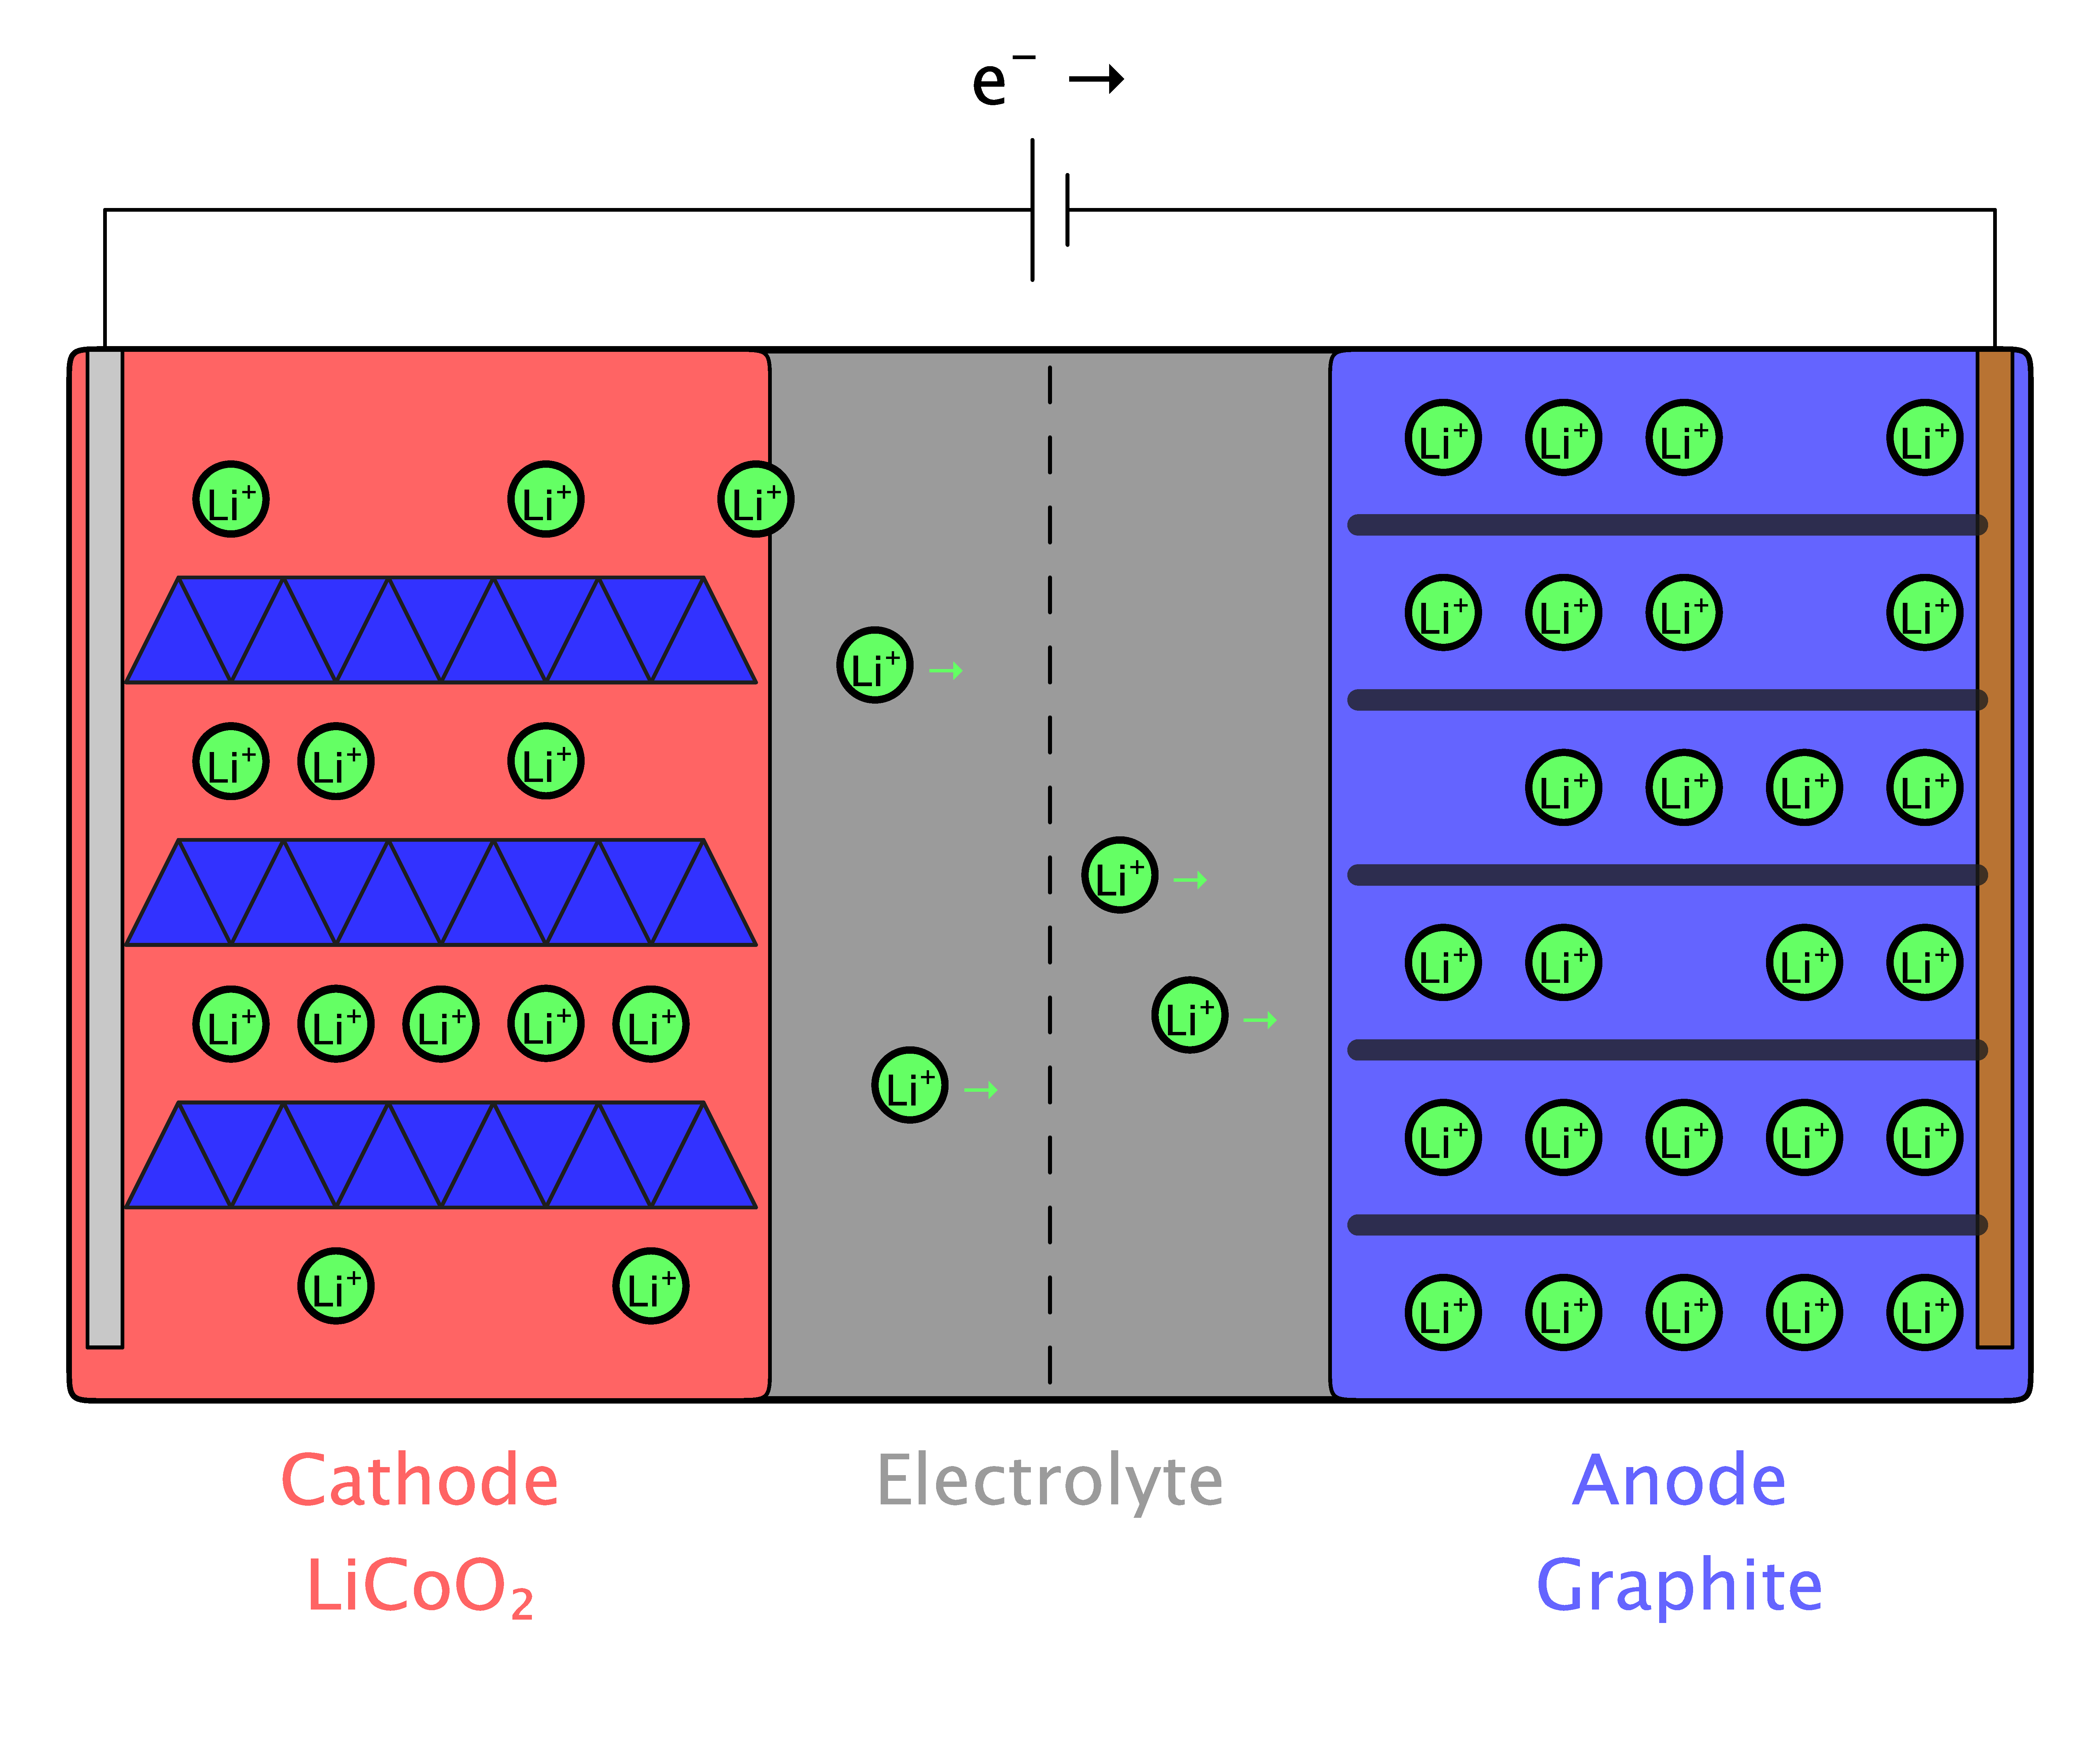
\includegraphics[width=0.7\linewidth, trim=1cm 1cm 1cm 1cm, clip]{figures/batteryCharge/batteryCharge}
  \caption{Charging}
  \label{fig:GoodenoughCharging}
\end{subfigure}

\begin{subfigure}{\linewidth}
  \centering
  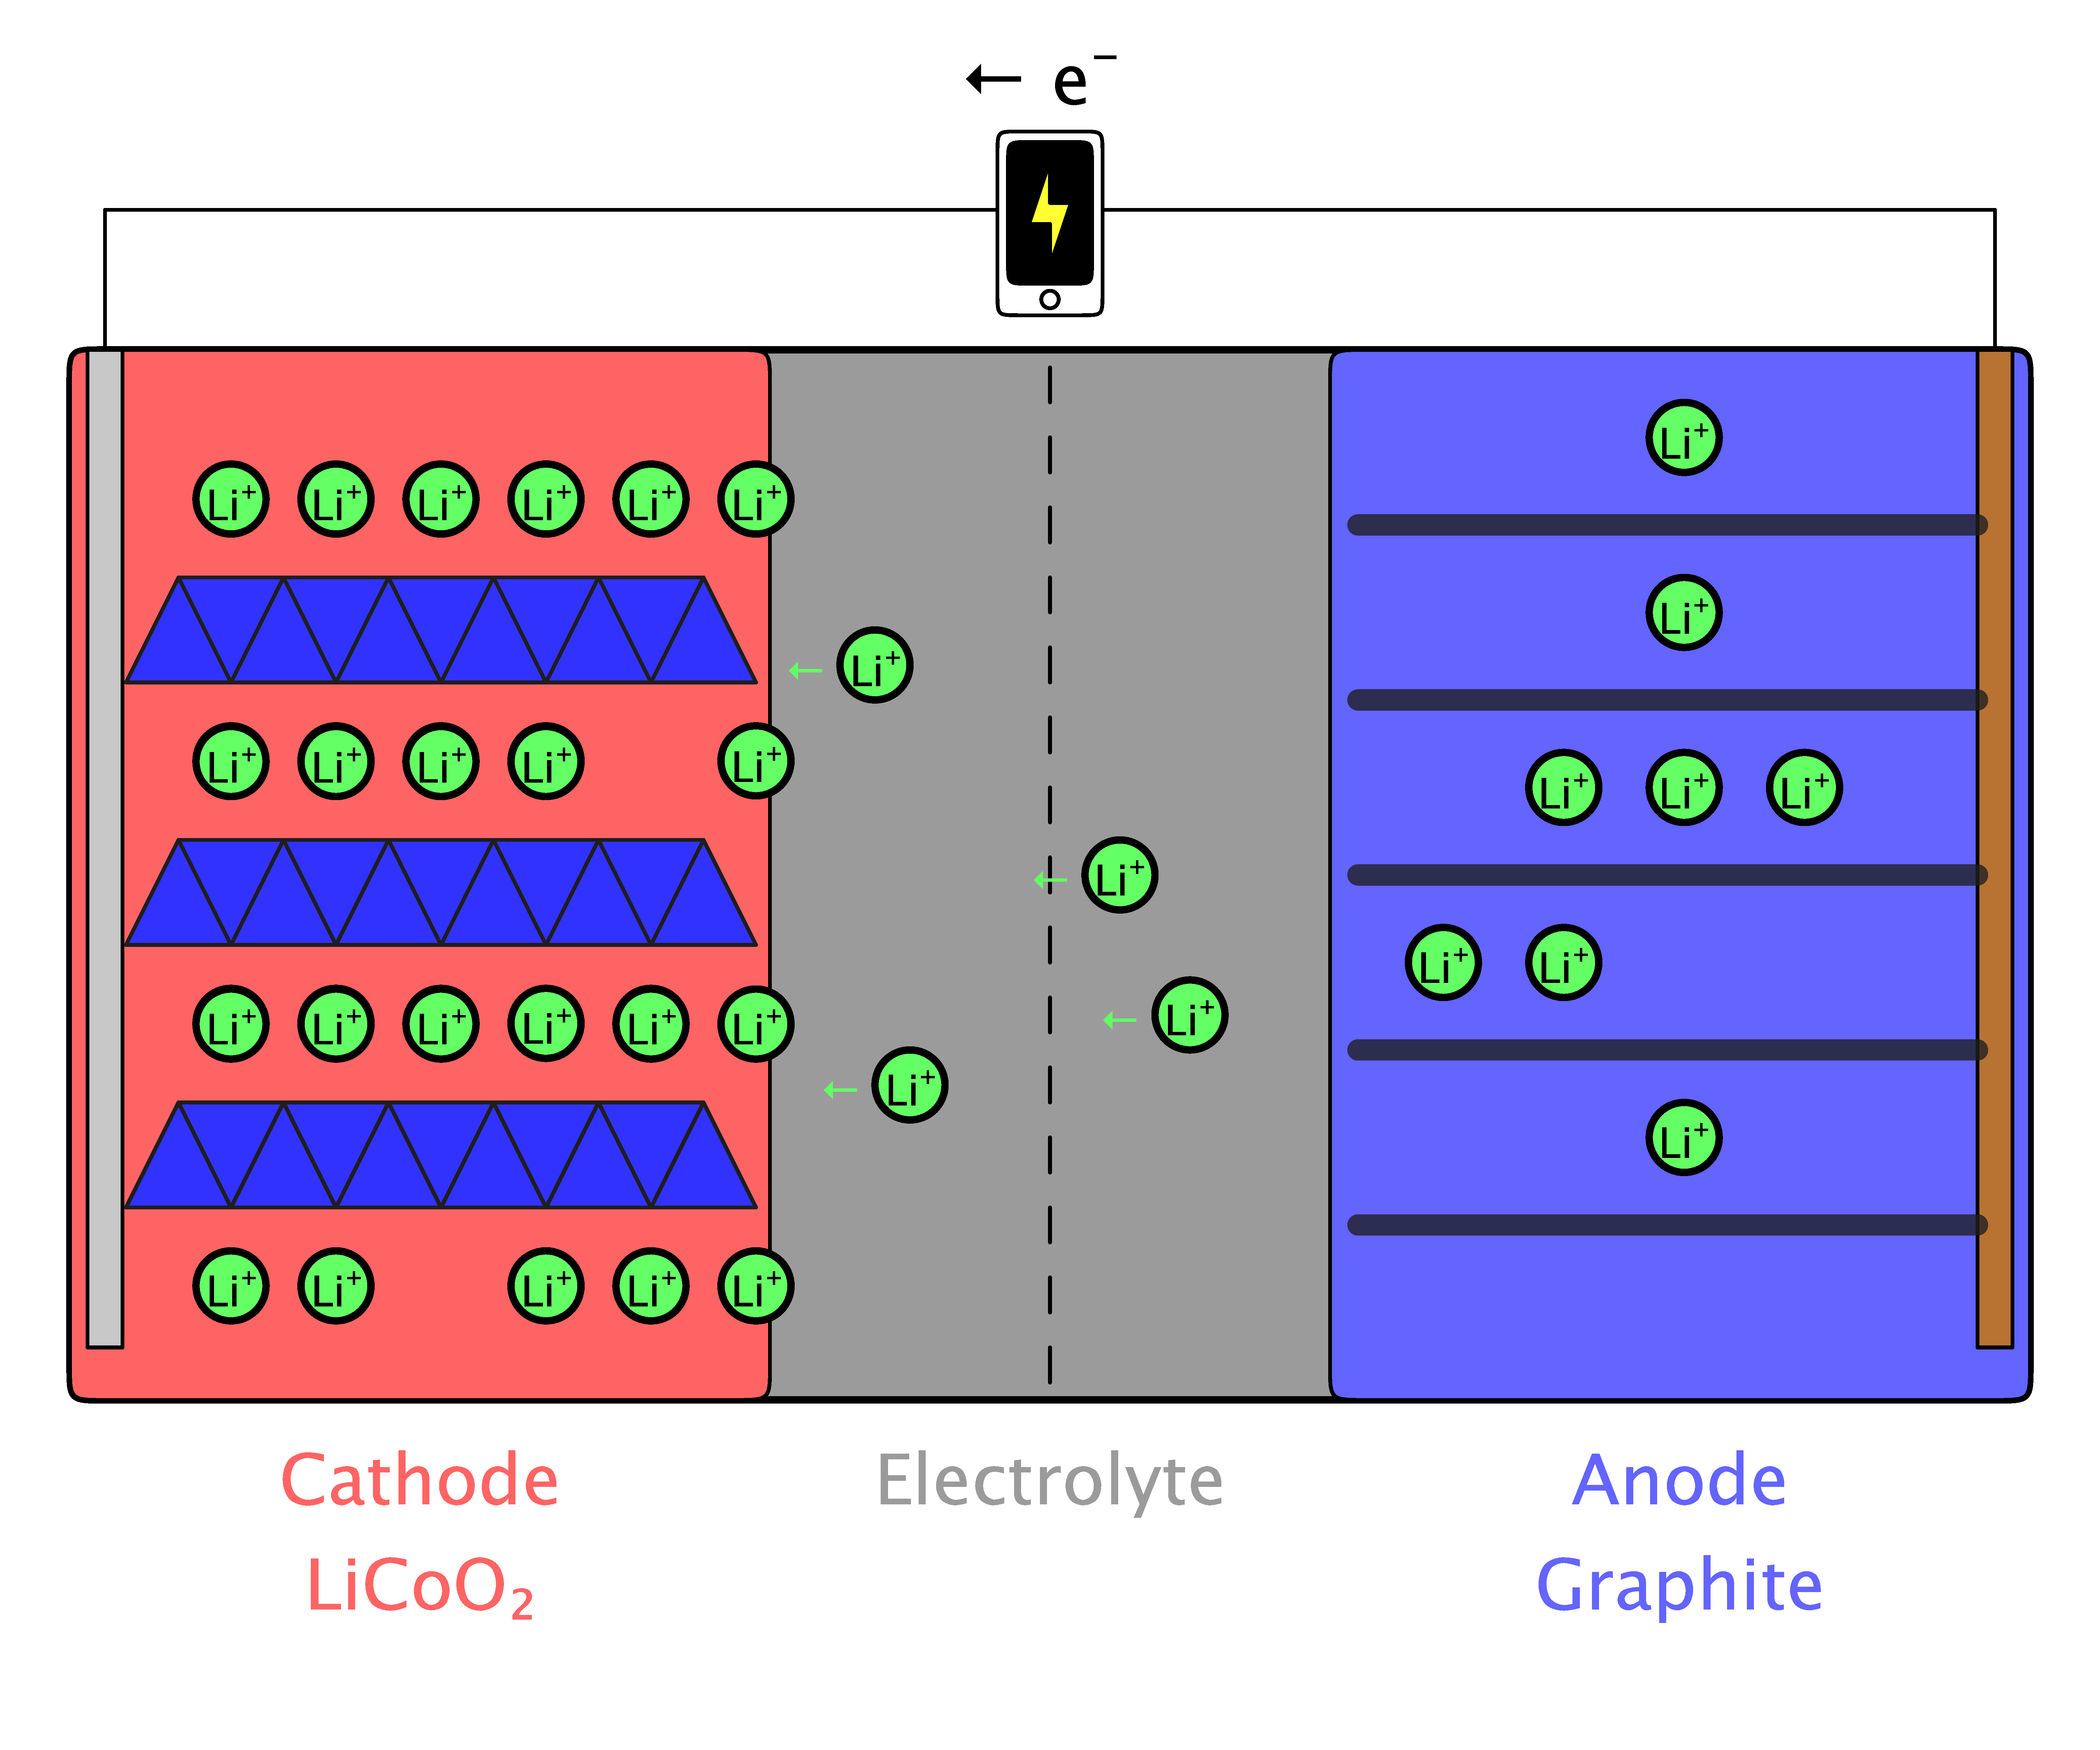
\includegraphics[width=0.7\linewidth, trim=1cm 1cm 1cm 1cm, clip]{figures/batteryDischarge/batteryDischarge}
  \caption{Discharging}
  \label{fig:GoodenoughDischarging}
\end{subfigure}
\caption[Li-ion battery schematic]{A schematic of a common Li-ion battery. During charging (a), electrons are driven to the anode by an external potential. \ce{Li+} ions move from the cathode to the anode to charge balance. During discharge (b), \ce{Li+} ions are driven to the cathode by a difference in chemical potential. The electrodes are electrically isolated by the separator, and are forced to instead travel via an external circuit and provide work.} 
\label{fig:Goodenough}
\end{figure}

\newpage
\section{Electrolyte materials}
In order for useful work to be yielded from batteries, and in order to prevent short circuiting, the electrodes must be electrically isolated from one another.
In practice, this is implemented by use of a porous but electrically insulating separator material (typically a multilayer polymer) coupled with an electrolyte material.
As the rate at which the battery can discharge is dependant on the rate at which the electrodes can exchange \ce{Li+} ions, high ionic conductivity is a vital for commercially viable electrolytes.


\subsection{Liquid electrolytes}
All Li-ion battery systems currently available commercially use liquid electrolytes.\cite{Famprikis2019}
These typically consist of \ce{LiFP6} salts dissolved in a mixture of organic solvents.
The exact composition will vary dependant on the choice of electrodes, application, and manufacturer.
That said, the use of ethyl methyl carbonate (EC) is universal in organic electrolytes, as its inclusion results in the formation of a passivating layer on graphite anodes, preventing solvent molecules from intercalating into the anode and destroying the graphitic structure.

These electrolyte solutions are typically stable to \SI{3.5}{\volt}, above which the electrolyte decomposes in a kinetically limited process.\cite{Palacin2009a}
As conventional batteries are often charged above \SI{3.5}{\volt}, this causes a slow decline in the performance of the battery over time.
The use of hierarchical electrode materials may mitigate this issue and allow the use of higher voltage cathode chemistries. \cite{Zhou2018}

\subsection{Solid electrolytes}
Solid-state batteries have been of significant research interest in recent years, primarily due to the increased safety they can offer.\cite{Famprikis2019, Zhang2018, Manthiram2017a, Janek2016}
Liquid electrolytes typically consist of highly flammable organic solvents which lead to dangerous failure modes.
The use of such electrolytes in EV applications, where mechanical failure of batteries is likely in the event of a crash, can significantly enhance the safety of EV's.

They can also offer higher energy densities, by enabling the use of higher energy density electrode materials which cannot be in liquid electrolyte systems.
In particular, they may allow the use of Li-metal anodes (see Section \ref{sec:anodes}), increasing the energy density of the anode by an order of magnitude,\cite{Zhang2018} and high voltage cathode materials for which no stable liquid electrolyte exists.
\newpage
\section{Anode materials}
\label{sec:anodes}
Li metal is theoretically the best possible anode material with a huge theoretical capacity (\SI{3860}{\milli\ampere\hour\per\gram}/\SI{2061}{\milli\ampere\hour\per\centi\meter\cubed}), and was used in early Li battery research. 
Unfortunately, dendrite formation at the anode surface ultimately leads to short circuiting and fires, preventing its use with current commercially viable electrolytes. \cite{Cheng2017,Guo2017a,Lin2017}
As such, current commercial batteries generally use a graphitic anode which undergoes the following reversible reaction:
\begin{equation}
\ce{Li_xC6(s) <-> $x$Li+(soln) +6C(s) + $x$e-}
\end{equation}
The performance of graphite anodes is a function of their morphology, meaning the capacity achieved is strongly influenced by the manufacturing processes used and the state of health of the battery.
That said, 
The use of carbon (albeit value-added carbon) as key material in batteries is of course a huge advantage due to its high abundance, low cost, and excellent electrical conductivity.
Whilst the graphite anodes are not the current limiting factor in commercial batteries, having higher capacities (\SI{372}{\milli\ampere\hour\per\gram}) than the best available cathodes, they are still of research interest in anticipation of next-generation cathodes.

Tin and silicon based alloys offer higher capacities than graphite, but are currently not viable due to myriad issues including large volume changes (+200\% for Si) over a charge/discharge cycle.\cite{Scrosati2011}

\newpage
\section{Cathode materials}
Cathode materials are currently the limiting factor in commercial batteries, making them a highly active and rapidly changing field of research.
While a wide range of materials are currently of research interest, only a few classes of cathode materials have enjoyed widespread commercialisation thus far.

\subsection{\ce{LiMO2}}
\begin{figure}
\centering
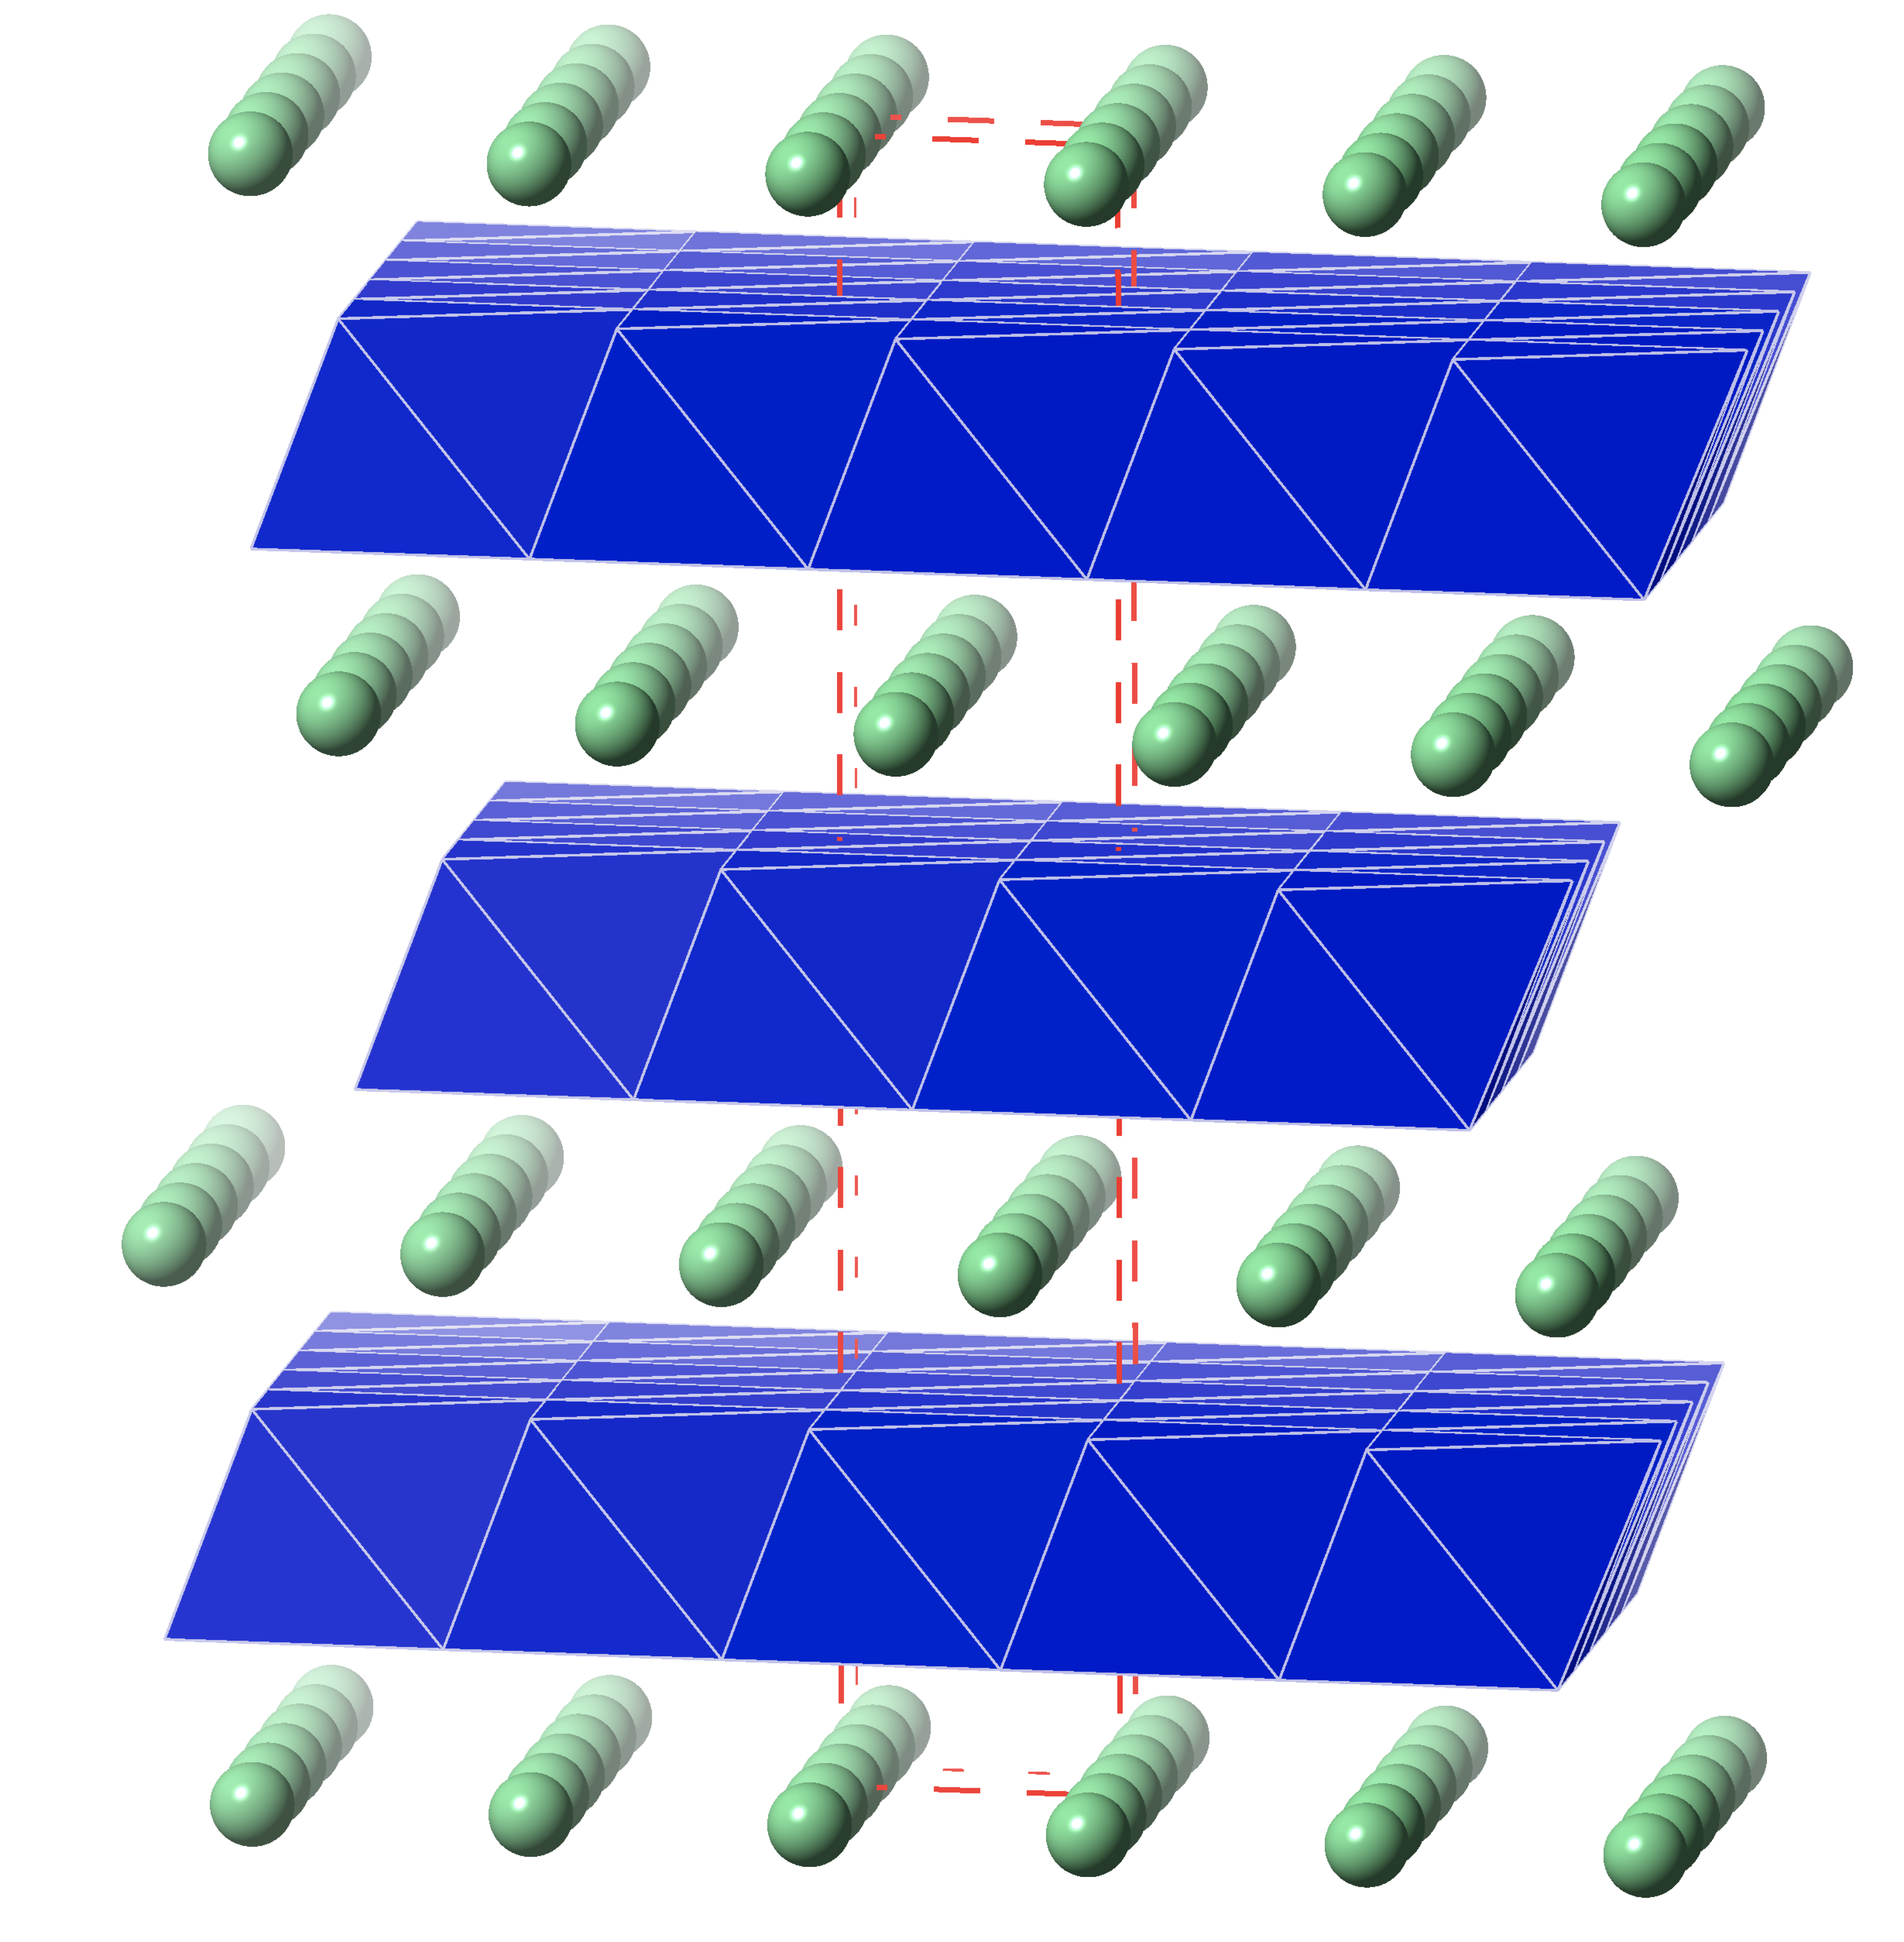
\includegraphics[width=\linewidth]{figures/structures/LiCoO2}
\caption[\ce{LiCoO2} structure]{\ce{LiCoO2} structure. (\ce{Li+} ions: green; \ce{MO6} octohedra: blue)\\ {\color{red} Work out a way of generating vectorised images for structures BEFORE wasting time making a ton of figures!}}
\label{fig:LCO}
\end{figure}
\ce{LiMO2} adopt \ce{\alpha-NaFeO2} structures (Figure \ref{fig:LCO}), which is the prototype structure of \ce{AMO2} layered cathode materials.
It adopts a structure with alternating layers of \ce{[CoO2]-} and \ce{Li+} layers ($R\bar{3}M$).\cite{Islam2014}
The low migration barrier between adjacent \ce{Li+} sites within each layer leads to fast 2D ion transport through the structure.
The reaction occurring as lithium is reversibly extracted from \ce{LiMO2} cathodes can be written as:\cite{Islam2014}
\begin{equation}
\ce{Li_{1-x}MO2(s) +$x$Li+(soln) +$x$e- <=> LiMO2(s)}
\end{equation}

Different metals allow for a larger fraction of Li to be reversibly extracted, corresponding to higher energy densities.





Li-air


\section{Li-rich cathodes}

Motivation, definition.

Anion redox. \cite{Yahia2019}


\subsection{Li2MnO3}

\subsection{Li-rich NMC}

\subsection{Li4Mn2O5}
\subsection{Li2MnO2F}




